\documentclass[11pt]{standalone}
\usepackage{tikz, pgfplots,amsmath, amssymb, amsthm}   
\usepgfplotslibrary{groupplots}


\begin{document}







\tikzset{every picture/.style={line width=0.75pt}} %set default line width to 0.75pt        

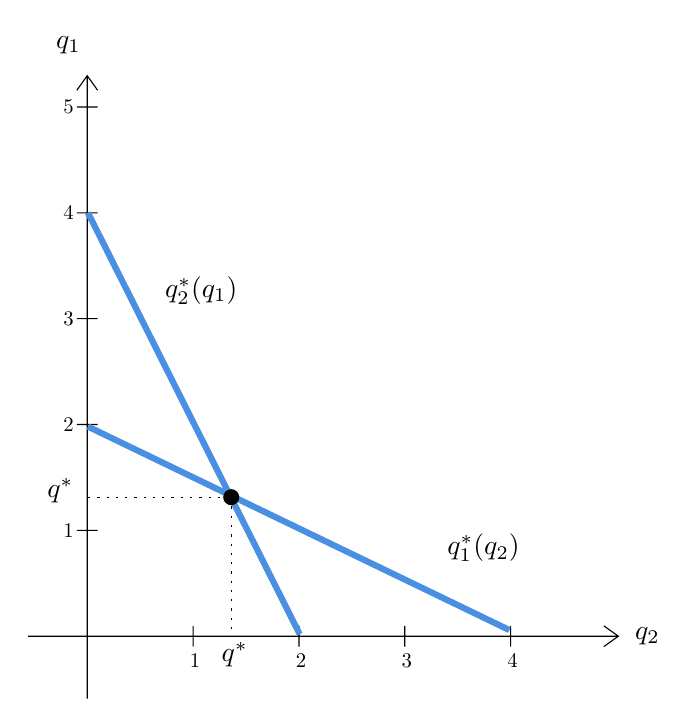
\begin{tikzpicture}[x=0.75pt,y=0.75pt,yscale=-1,xscale=1]
%uncomment if require: \path (0,357); %set diagram left start at 0, and has height of 357

%Shape: Axis 2D [id:dp8249355413689539] 
\draw  (116.5,328.99) -- (400.81,328.99)(144.93,58.93) -- (144.93,359) (393.81,323.99) -- (400.81,328.99) -- (393.81,333.99) (139.93,65.93) -- (144.93,58.93) -- (149.93,65.93) (195.93,323.99) -- (195.93,333.99)(246.93,323.99) -- (246.93,333.99)(297.93,323.99) -- (297.93,333.99)(348.93,323.99) -- (348.93,333.99)(139.93,277.99) -- (149.93,277.99)(139.93,226.99) -- (149.93,226.99)(139.93,175.99) -- (149.93,175.99)(139.93,124.99) -- (149.93,124.99)(139.93,73.99) -- (149.93,73.99) ;
\draw   (202.93,340.99) node[anchor=east, scale=0.75]{1} (253.93,340.99) node[anchor=east, scale=0.75]{2} (304.93,340.99) node[anchor=east, scale=0.75]{3} (355.93,340.99) node[anchor=east, scale=0.75]{4} (141.93,277.99) node[anchor=east, scale=0.75]{1} (141.93,226.99) node[anchor=east, scale=0.75]{2} (141.93,175.99) node[anchor=east, scale=0.75]{3} (141.93,124.99) node[anchor=east, scale=0.75]{4} (141.93,73.99) node[anchor=east, scale=0.75]{5} ;
%Straight Lines [id:da27745455225430904] 
\draw [color={rgb, 255:red, 74; green, 144; blue, 226 }  ,draw opacity=1 ][line width=2.25]    (145.3,125) -- (247.3,328) ;


%Straight Lines [id:da4756245979691436] 
\draw [color={rgb, 255:red, 74; green, 144; blue, 226 }  ,draw opacity=1 ][line width=2.25]    (145.3,228) -- (348.3,326) ;


%Straight Lines [id:da45087630940110657] 
\draw  [dash pattern={on 0.84pt off 2.51pt}]  (145.3,262) -- (214.3,262) ;
\draw [shift={(214.3,262)}, rotate = 0] [color={rgb, 255:red, 0; green, 0; blue, 0 }  ][fill={rgb, 255:red, 0; green, 0; blue, 0 }  ][line width=0.75]      (0, 0) circle [x radius= 3.35, y radius= 3.35]   ;

%Straight Lines [id:da6366621561129924] 
\draw  [dash pattern={on 0.84pt off 2.51pt}]  (214.3,262) -- (214.3,329) ;



% Text Node
\draw (199.85,162.47) node [color={rgb, 255:red, 0; green, 0; blue, 0 }  ,opacity=1 ]  {$q^{*}_{2}( q_{1})$};
% Text Node
\draw (135.85,44.4) node   {$q_{1}$};
% Text Node
\draw (414.88,328.83) node   {$q_{2}$};
% Text Node
\draw (335.85,286.47) node [color={rgb, 255:red, 0; green, 0; blue, 0 }  ,opacity=1 ]  {$q^{*}_{1}( q_{2})$};
% Text Node
\draw (132,259) node   {$q^{*}$};
% Text Node
\draw (216,338) node   {$q^{*}$};


\end{tikzpicture}


\end{document}